% Copyright (c) 2021 Eclipse Arrowhead Project
%
% This program and the accompanying materials are made available under the
% terms of the Eclipse Public License 2.0 which is available at
% http://www.eclipse.org/legal/epl-2.0.
%
% SPDX-License-Identifier: EPL-2.0

For a document, \GlossaryHyperRef{model}{model}, or other \GlossaryHyperRef{artifact}{artifact}, to be allowed to claim conformance to \textit{this work}, the following must be observed by that \textit{derived work}:

\begin{enumerate}
\item At least one of the concepts defined in this work must be part of that derived work.
\item The derived work must make it explicit what concepts are taken from this work.
	\begin{enumerate}
	\item How this is done most suitably depends on the type of derived work. A document may include a normative reference to this document, while a model may want to give all relevant \GlossaryHyperRef{entity}{entities} and \GlossaryHyperRef{relationship}{relationships} an \GlossaryHyperRef{attribute}{attribute} with the identity of this document, for example.
	\end{enumerate}
\item Every concept taken from this work must be represented by the name it is given here.
	\begin{enumerate}
	\item If important to be able to distinguish an Arrowhead concept from other such of relevance, concepts from this work may be qualified by the leading word ``Arrowhead'', as in, for example, ``Arrowhead system`` or ``Arrowhead service function''.
	\item Note that some concepts defined here are given more than one name. In some cases one of these names may be designated as being preferred. Preferred names should be used by derived works. Whether or not a name is preferred is noted in the Glossary of Section \ref{sec:glossary} by it not referring to any other name as being preferred. If a referred name is designated as synonymous, it or any other name of the concept in question may be used.
	\end{enumerate}
\item Concepts taken from this work may be \textit{specialized} and/or \textit{simplified}, but must never be \textit{contradicted}.
	\begin{enumerate}
	\item \textit{Specialization} means that more \GlossaryHyperRef{constraint}{constraints} are applied to it than are presented here. For example, a certain derived work may require that all devices have \GlossaryHyperRef{unit-compute}{compute units} supporting a certain instruction set, or that every \GlossaryHyperRef{system}{system} \GlossaryHyperRef{provider-service}{provides} a specific monitoring \GlossaryHyperRef{service}{service}, and so on.
	\item \textit{Simplification} means that entities, relationships or attributes introduced here are omitted due to being outside the scope of the derived work. For example, a technical document may not be concerned with \GlossaryHyperRef{role-stakeholder}{stakeholder roles}, while a model of certain types of local clouds may not be concerned with whether or not artifacts are \GlossaryHyperRef{resource}{resources} or not, and so on.
	\item \textit{Contradiction} means that an attribute or other constraint is introduced that makes it impossible to reconcile the concepts presented here with those in the derived work. A derived work must not, for example, demand that no devices ever host systems. Contradictions generally only occur when some relationship or attribute is both demanded to exist and not to exist at the same time.
	\end{enumerate}
\item \label{sec:conformance:notation} If a different graph notation is used than the one described in Section \ref{sec:introduction:conventions:graphs}, the derived work must either describe how its notation maps to the notation here, or refer to a work making such a description.
	\begin{enumerate}
	\item The graph constructs that have to be mapped are as follows:
		\begin{enumerate}
		\item \textit{entities}, which are boxes with solid lines and names inside them;
		\item \textit{relationships}, which are unidirectional arrows with \textit{names} and \textit{quantifiers} that denote association;
		\item \textit{attributes}, which are special properties expressed in text only.
		\end{enumerate}
		Each relevant relationship name and attribute of this document must be mapped to an equivalent construct in the target notation.
	\item In practice, only text documents claiming to adhere to the graph diagram notation of Section \ref{sec:introduction:conventions:graphs} are exempt from having to describe or refer to such a notational mapping. As mappings to this document will be hard to produce rigorously without text, we expect all such mappings to be described in text documents.
	\end{enumerate}
\end{enumerate}

\newpage

\subsection{ISO/IEC/IEEE 42010}
\label{sec:conformance:iso42010}

The ISO42010 \cite{iso42010} standard provides a uniform way for system architects to produce architectural \GlossaryHyperRef{description}{descriptions}, \GlossaryHyperRef{viewpoint-architecture}{viewpoints}, \GlossaryHyperRef{framework-architecture}{frameworks} and \GlossaryHyperRef{language-architecture-description}{description languages}.
In the context of ISO42010, this work can be used as a \GlossaryHyperRef{metamodel}{\textit{metamodel}} part of an \GlossaryHyperRef{kind-model}{model kind}, as illustrated in Figure \ref{fig:iso42010}.

\begin{figure}[ht!]
  \centering
  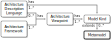
\includegraphics[scale=0.9]{figures/iso42010}
  \caption{
    The metamodel as a part of an ISO42010 model kind, which in turn may be referenced by architecture description languages and architecture frameworks.
  }
  \label{fig:iso42010}
\end{figure}

Using this work as a metamodel largely entails referencing a work that maps the concepts of this work to a relevant modeling language, as discussed in conformance requirement \ref{sec:conformance:notation}.
The mapping work must, of course, satisfy all conformance requirements outlined earlier in this section.
The use of metamodels is described more fully in Annex B, Section B.2.6 of ISO42010 \cite{iso42010}.
If you want to learn more about the standard and how to use it, please refer to the standard itself or other relevant learning resources\footnote{At the time of writing (2021-12-15), guides to ISO42010 were available at \url{http://www.iso-architecture.org/42010}.}.